\documentclass[UTF8]{article}
\pagestyle{plain}
\usepackage{graphicx}
\usepackage{subfigure}
\usepackage{ctex}
\usepackage{float}
\title{经济学科普: \\ 2.供给与需求}
\author{白纸}
\date{\today}
\begin{document}
\maketitle

\section{参考内容}
    徐高,《宏观经济学二十五讲:中国视角》\par
    曼昆,《微观经济学原理》第4章:供给和需求的市场力量\par
    费雪,《利息理论》第1章:收入与资本

\section{供给与需求的简介}
    在曼昆的《微观经济学原理》第4章:供给和需求的市场力量,对供给和需求有详细清晰的描述。
    简单地说,供给和需求是推动市场经济运行的力量,决定了每种商品的产量和销售价格。\par
    某种商品的需求量是买者愿意且有能力购买的数量,某种商品(服务)的供给量是卖方愿意且有能力出售的数量。
    对于买者,需求量被什么因素影响呢?对于卖者,供给量被什么因素影响呢?
    
    \subsection{直接因素}
        直接因素,就是价格,价格就是自变量。
        对于买者,某种商品价格升高,需求量下降;价格降低,需求量上升。
        对于卖者,某种商品价格升高,供给量上升;价格降低,供给量下降。\par
        要注意的是:在数学中,我们一般把自变量放在横轴,
        但是在经济学中,价格作为自变量,一般被放在纵轴。
%        \begin{figure}[H]
%            \centering
%            \subfigure[供给曲线] {
%                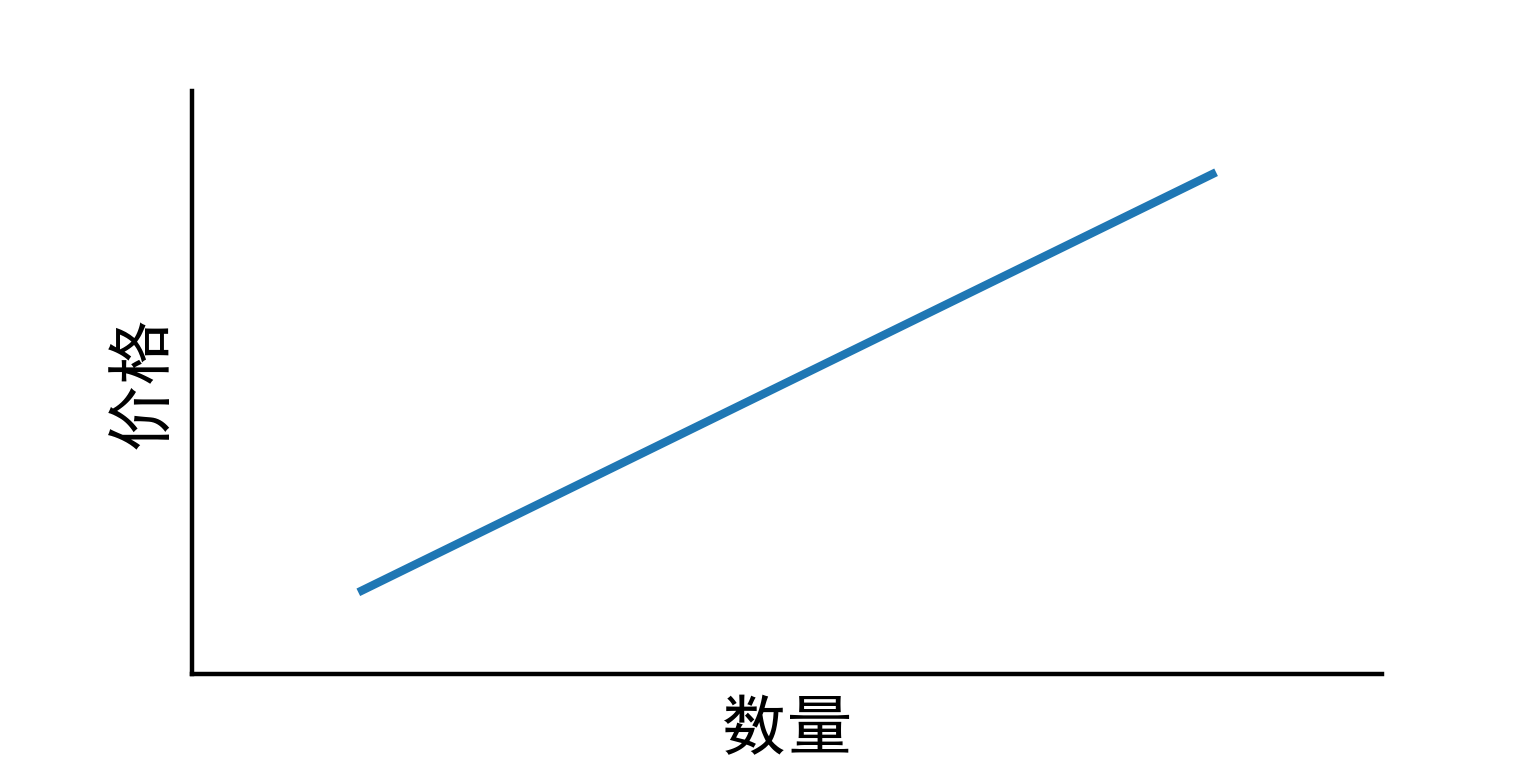
\includegraphics[width = 5.5cm]{供给曲线.png}
%            }
%            \quad
%            \subfigure[需求曲线] {
%                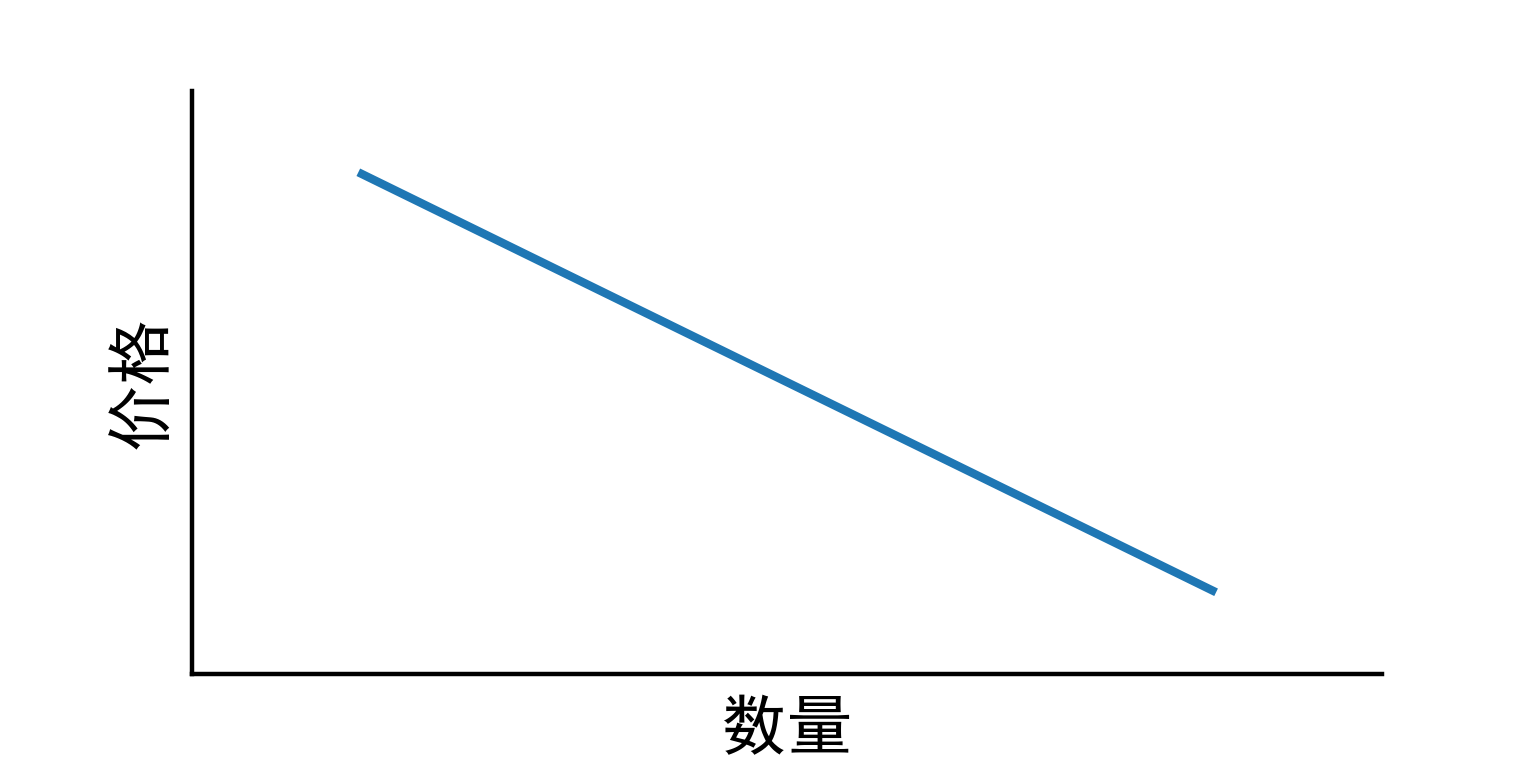
\includegraphics[width = 5.5cm]{需求曲线.png}
%            }
%        \end{figure}
        \begin{figure}[H]
            \centering
            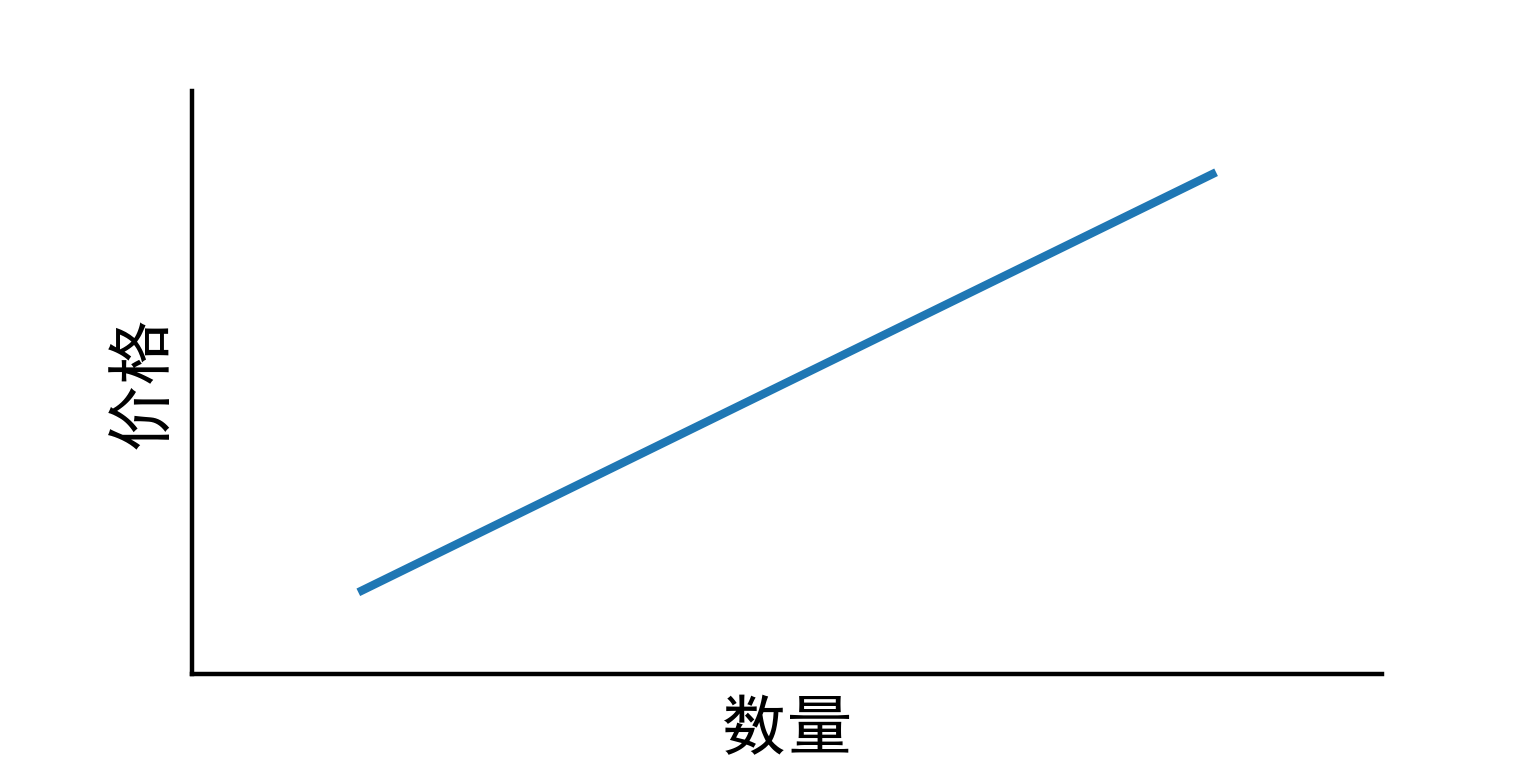
\includegraphics[width = 1 \textwidth]{供给曲线.png}
            \caption{供给曲线}
        \end{figure}
        \begin{figure}[H]
            \centering
            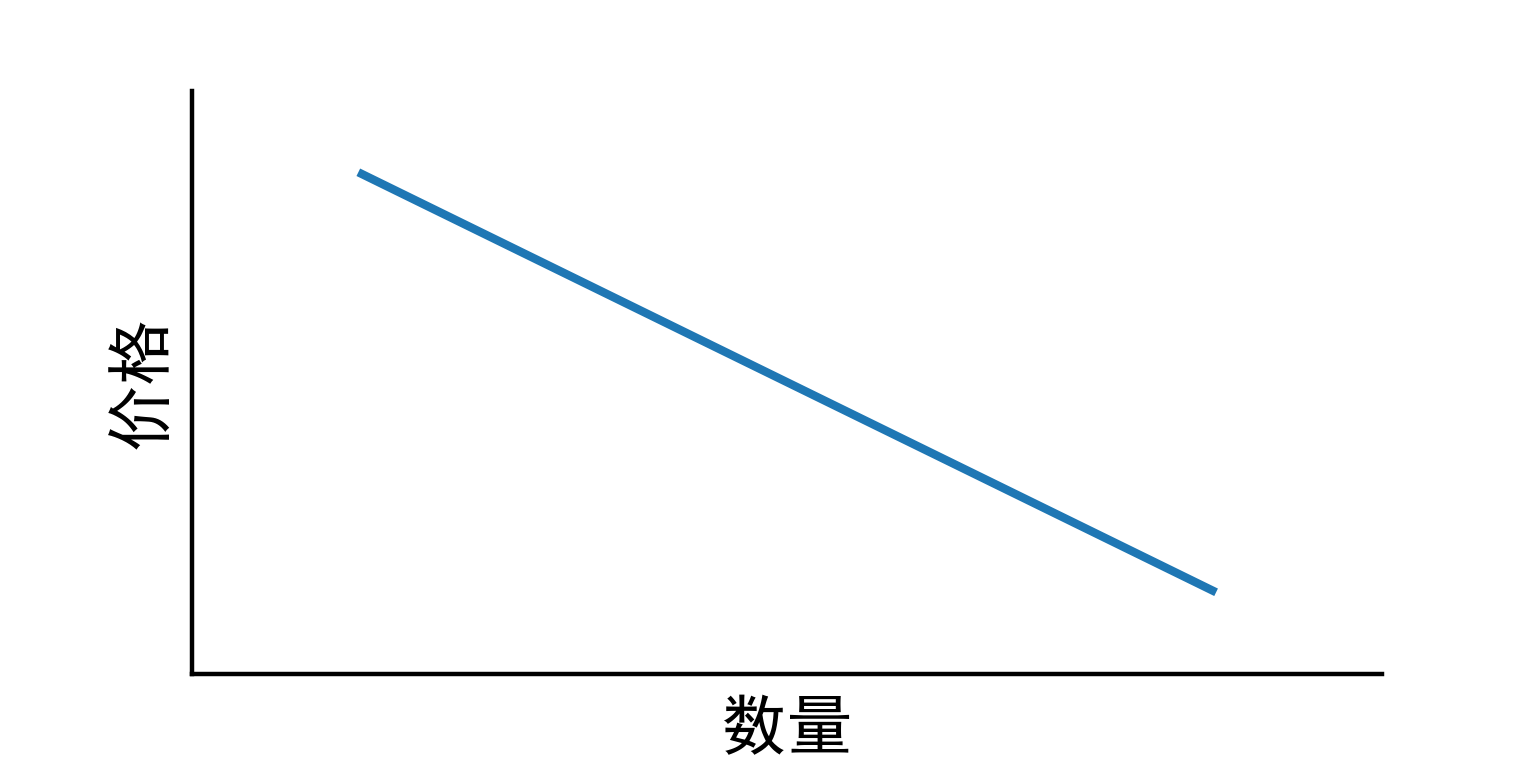
\includegraphics[width = 1 \textwidth]{需求曲线.png}
            \caption{需求曲线}
        \end{figure}

    \subsection{间接因素}

\end{document}
